\chapter{Конструкторский раздел}

В данном разделе сформулированы требования и ограничения к разрабатываемому методу. Разработан метод восстановления дефокусированных изображений на основе определенных параметров искажения. Описаны основные этапы разработки в виде детализированной диаграммы IDEF0 и схем алгоритмов, а также изложены особенности излагаемого метода. Спроектировано программное обеспечение для реализации разрабатываемого метода.

\section{Требования и ограничения к разрабатываемому методу}

К методу восстановления дефокусированных изображений на основе определенных параметров предъявляются следующие требования:

\begin{enumerate}
	\item Определять параметр искажения (радиус дефокусировки).
	\item Определять функцию рассеяния точки, которая была применена к искаженному изображению.
	\item Восстанавливать искаженное изображение с использованием ФРТ.
\end{enumerate}

Также представлен ряд ограничений для разрабатываемого метода:

\begin{enumerate}
	\item Качество восстановления может быть неудовлетворительным, если изображение было подвергнуто существенному сжатию.
	\item Качество восстановления может быть неудовлетворительным, если изображение с высоким уровнем шума и/или имеет высокочастотные детали (выбросы интенсивности).
\end{enumerate}

Не предполагается обработка изображений c частичной дефокусировкой, т.е. когда искажение присутствует только в определенной области, а не распространяется на всю площадь. Для обработки дефокусировки в этом случае можно выделить часть необходимую изображения. Не предполагается обработка заведомо недефокусированных изображений. Не предполагается повторое применение метода к изображению.

Также естественным ограничением семейства методов деконволюции (как <<слепой>>, так и классической) является тот факт, что чем сильнее искажение (больше радиус дефокусировки), тем менее эффективен метод, т.к. дефокусировка является лишь частично обратимым процессом. Это связано с тем, что при увеличении силы влияния искажения теряется снижается количество информации на изображении.

\section{Требования к разрабатываемому программному обеспечению}

К разрабатываемому программному обеспечению предъявляются следующие требования:

\begin{enumerate}
	\item Возможность загрузки изображений в формате PNG, JPG или BMP.
	\item Возможность обработки как RGB~--~изображений, так и изображений в тонах серого.
	\item Возможность просмотра результата восстановления в сравнении с исходным изображением.
	\item Возможность сохранения результата в отдельный файл в формате PNG, JPG или BMP.
	\item Если время выполнения программы может превышать комфортное время реакции системы для человека, необходимо обеспечить вывод предупреждающего сообщения. 
	\item Разрабатываемое ПО должно корректно реагировать на любые действия пользователя.
\end{enumerate}

\clearpage

\section{Основные этапы разрабатываемого метода}

\subsection{IDEF-0 диаграмма уровня А1}

На рисунке \ref{idef0-a1} представлена диаграмма IDEF0 уровня А1 для разрабатываемого метода.

\begin{figure}[H]
	\centering
	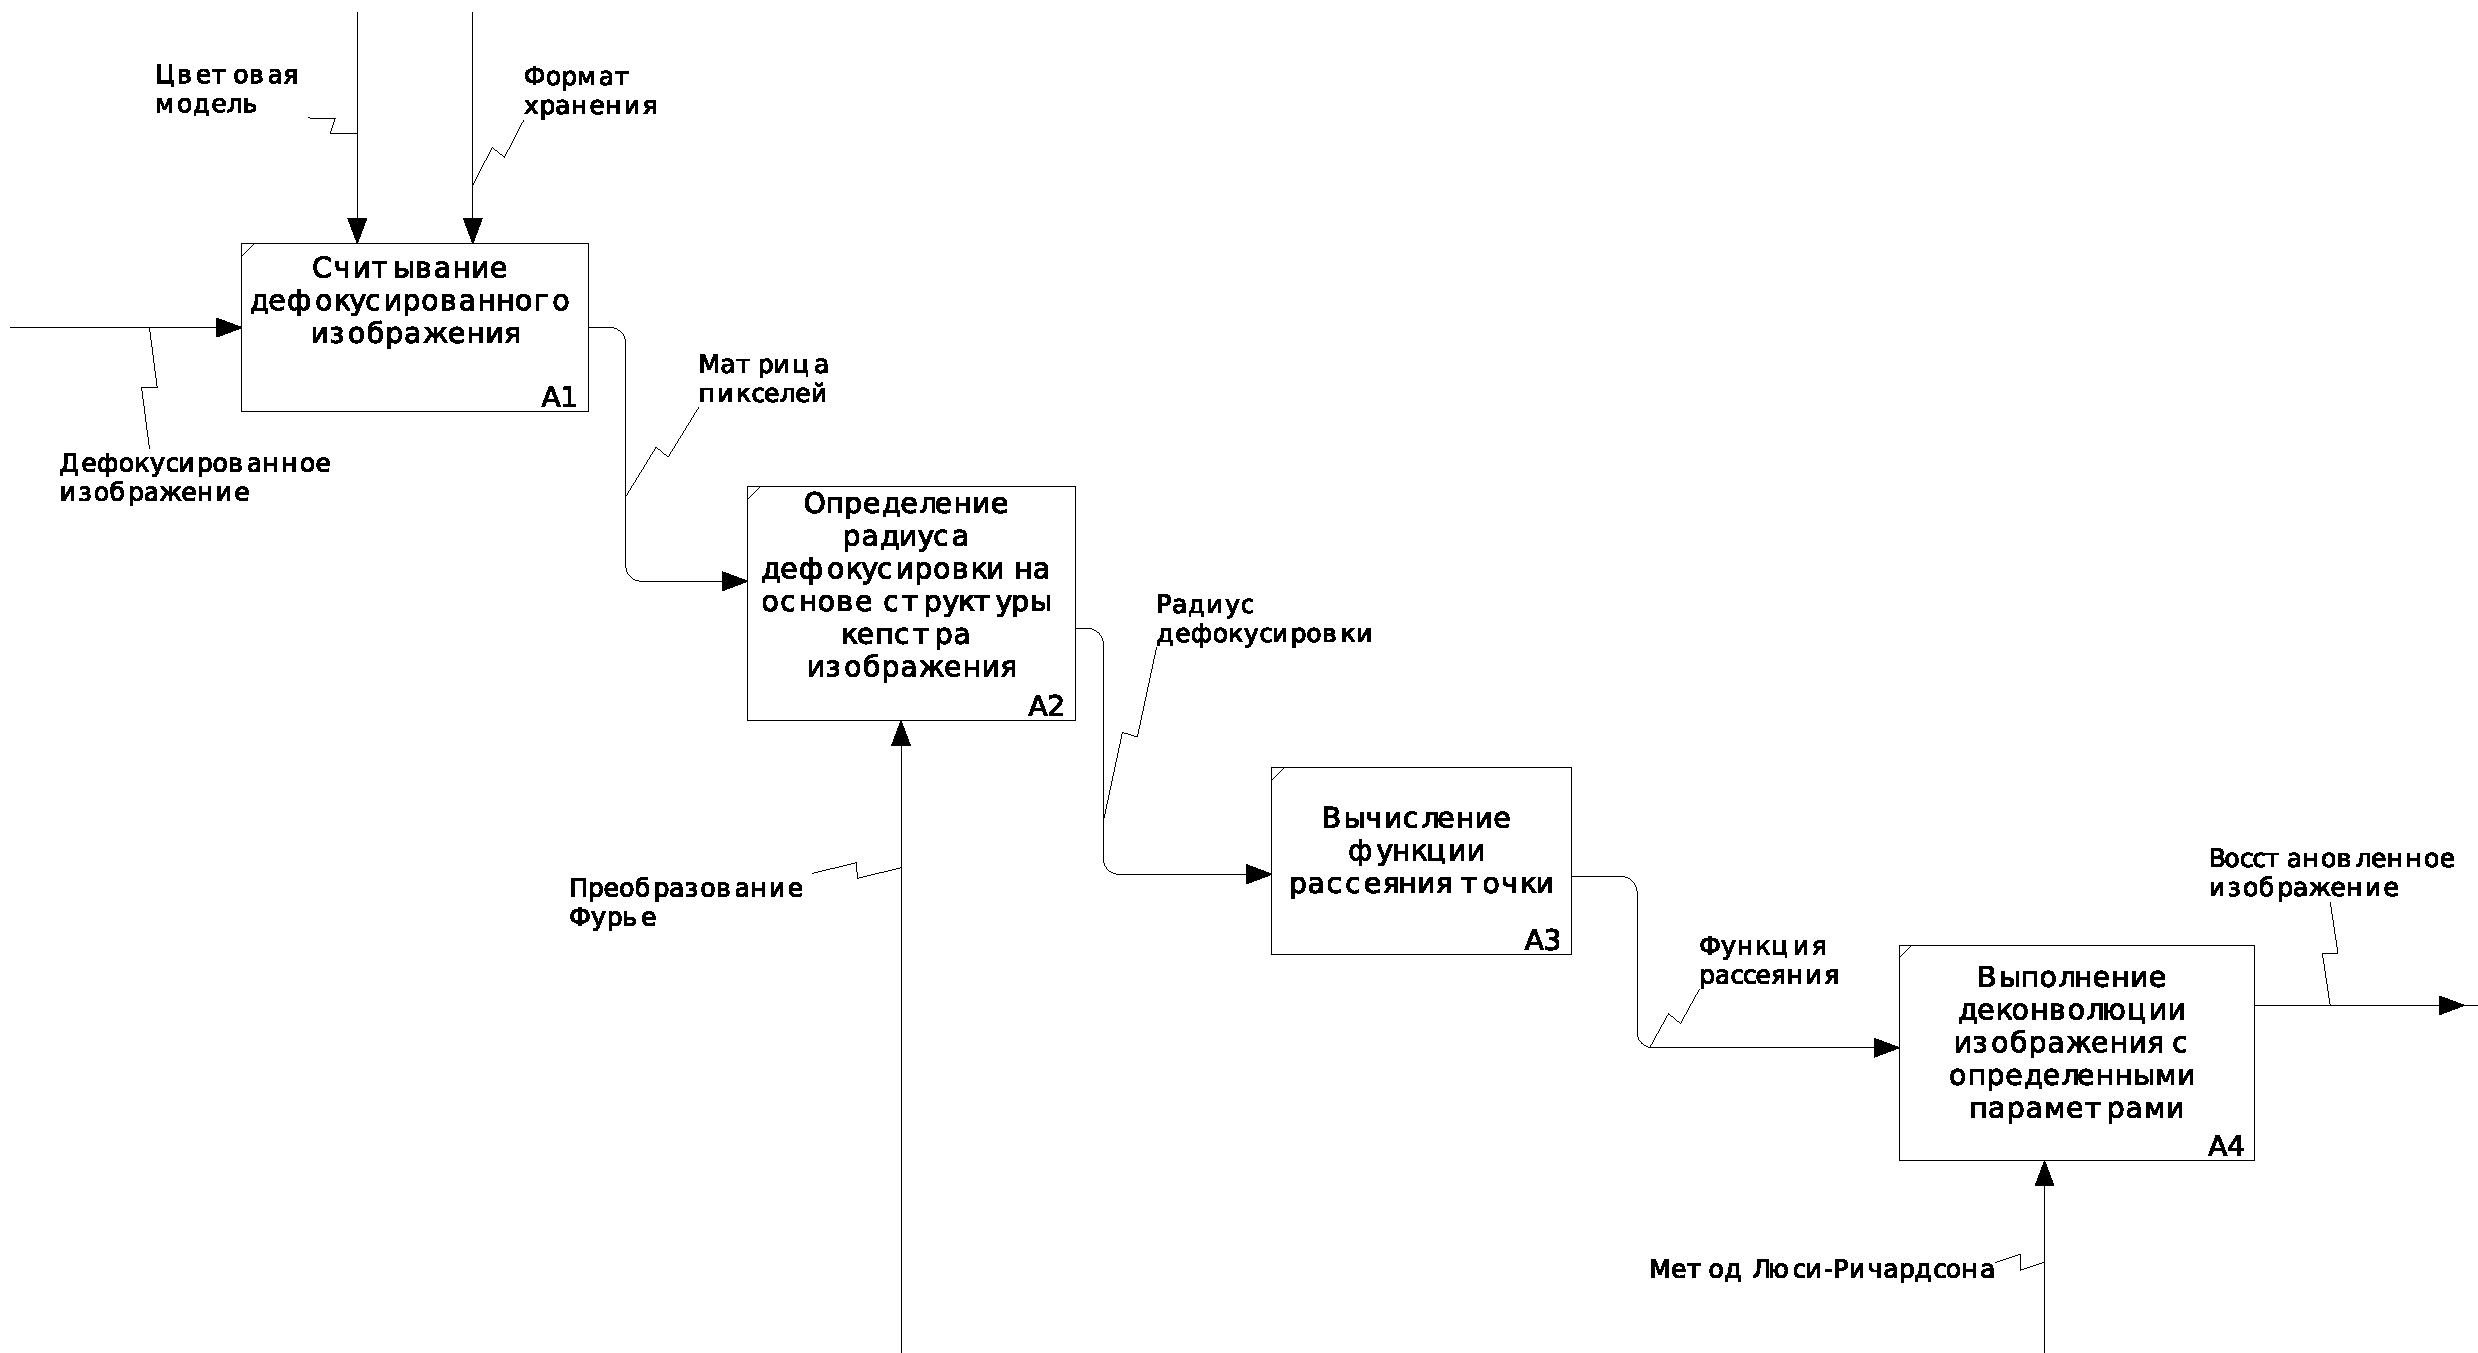
\includegraphics[scale=0.4]{assets/02_A0}
	\caption{IDEF0~--~диаграмма уровня А1}
	\label{idef0-a1}
\end{figure}

\subsection{Схемы алгоритмов} 

На \textit{первом} этапе исходное дефокусированное изображение считывается в матрицу пикселей, с которой в дальнейшем будут происходить все вычисления. В соответствии с требованиями, изображение может одноканальным (grayscale) или трехканальным (RGB). В первом случае все действия производятся однократно, во втором~---~необходимо воспроизвести соответствующие вычисления для каждого из каналов, а затем результат объединить в трехканальное изображение.

На \textit{втором} этапе происходит определение радиуса дефокусировки на основе структуры кепстра изображения. Основная идея предлагаемого метода заключается именно в этом этапе.

На рисунке \ref{r=15} представлена схема, демонстрирующая влияние радиуса на данную структуру. В соответствии с этой закономерностью решено вычислять радиус дефокусировки как отношение радиуса ближайшего к центру кольца к размеру радиального профиля, равного половине ширины изображения.

\begin{figure}[H]
	\centering
	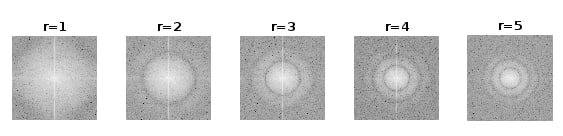
\includegraphics[scale=0.9]{assets/r15.jpg}
	\caption{Влияние радиуса дефокусировки на структуру кепстра изображения}
	\label{r=15}
\end{figure}

На рисунке \ref{cepstrum} представлен алгоритм вычисления кепстра.

\begin{figure}[H]
	\centering
	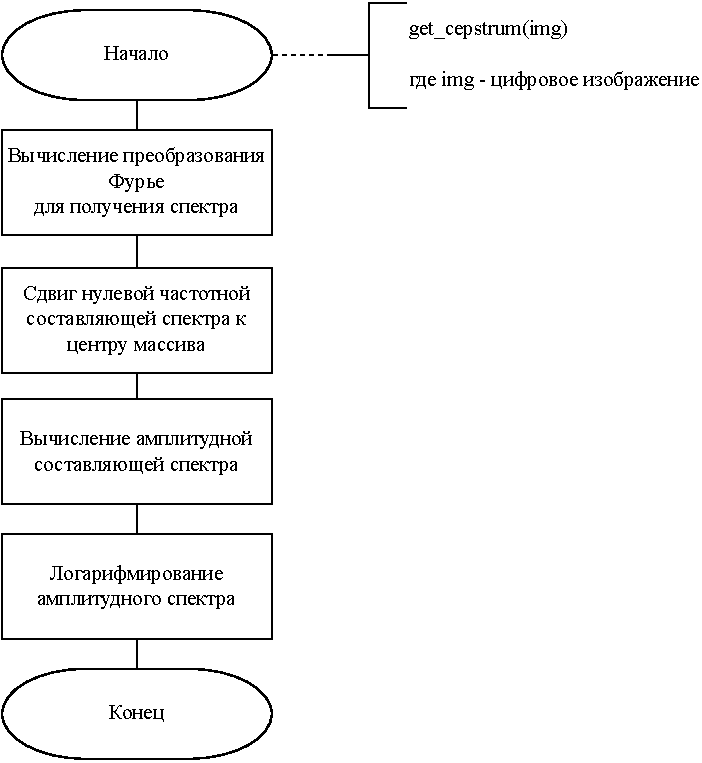
\includegraphics[scale=1]{assets/cepstrum.pdf}
	\caption{Алгоритм вычисления кепстра изображения}
	\label{cepstrum}
\end{figure}

Сдвиг нулевой частотной составляющей необходим для удобства восприятия полученной структуры. Логарифмирование кепстра производится также с целью повышения качества визуального восприятия. Для получения амплитудной составляющей необходимо вычислить модуль кепстра. %обратное ПФ нужно ли?

На рисунке \ref{radius} представлен алгоритм вычисления радиуса дефокусировки на основе кепстрального анализа.

\begin{figure}[H]
	\centering
	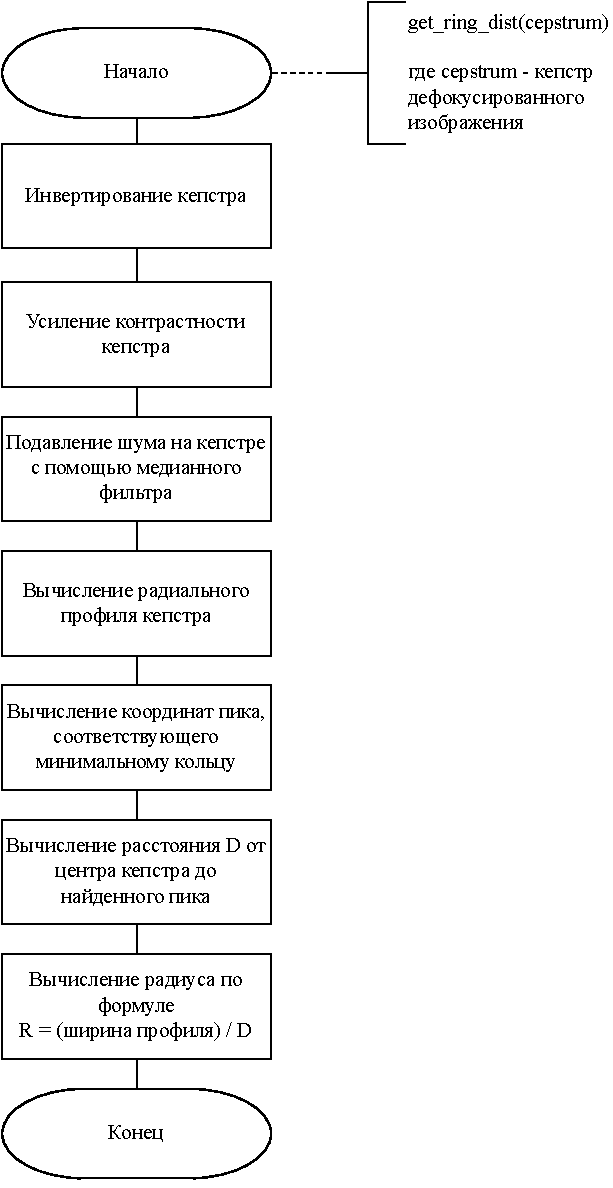
\includegraphics[scale=0.9]{assets/radius.pdf}
	\caption{Алгоритм вычисления радиуса дефокусировки}
	\label{radius}
\end{figure}

В рамках этого этапа входным параметром является матрица пикселей, выходным --- радиус дефокусировки.

Инвертирование кепстра выполняется по причине того, что большинство средств обработки сигналов предоставляет широкий набор обработки пиков (максимумов) интенсивности. 

Усиление контрастности проводится с целью повышения точности распознавания радиуса кольца кепстра. 

Применение медианного фильтра позволяет подавить шум на изображении, сгладив помеху типа <<соль~-~перец>> в центре кепстра. Размер окна выбран так, чтобы не потерять информацию о деталях наблюдаемой структуры.

На \textit{третьем} этапе метода составляется функция рассеяния точки, описывающая процесс искажения, на основе определенного на предыдущем этапе радиуса дефокусировки. Данная матрица имеет тип квадратной матрицы размером, равным радиусу. 

В данный квадрат вписан круг радиусом, также равным двойному радиусу дефокусировки. Для ячеек матрицы, принадлежащих этому кругу, значение интенсивности вычисляется как $\cfrac{1}{\pi r^2}$, где $r$ --- радиус. Для остальных ячеек матрицы значение интенсивности равно 0.

На рисунке \ref{disk} представлен общий вид функции рассеяния точки.

\begin{figure}[H]
	\centering
	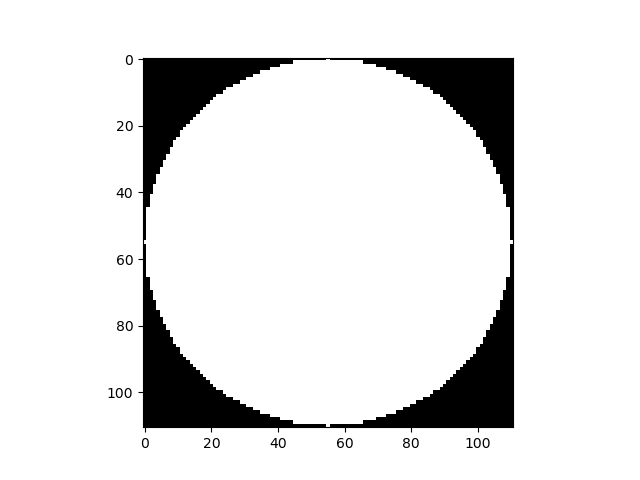
\includegraphics[scale=0.7]{assets/disk.png}
	\caption{Общий вид ФРТ}
	\label{disk}
\end{figure}

В рамках этого этапа входным параметром является радиус дефокусировки, выходным --- квадратная матрица пикселей, описывающая ФРТ заданного радиуса.

\clearpage

На рисунке \ref{psf} представлен алгоритм вычисления ФРТ на основе радиуса.

\begin{figure}[H]
	\centering
	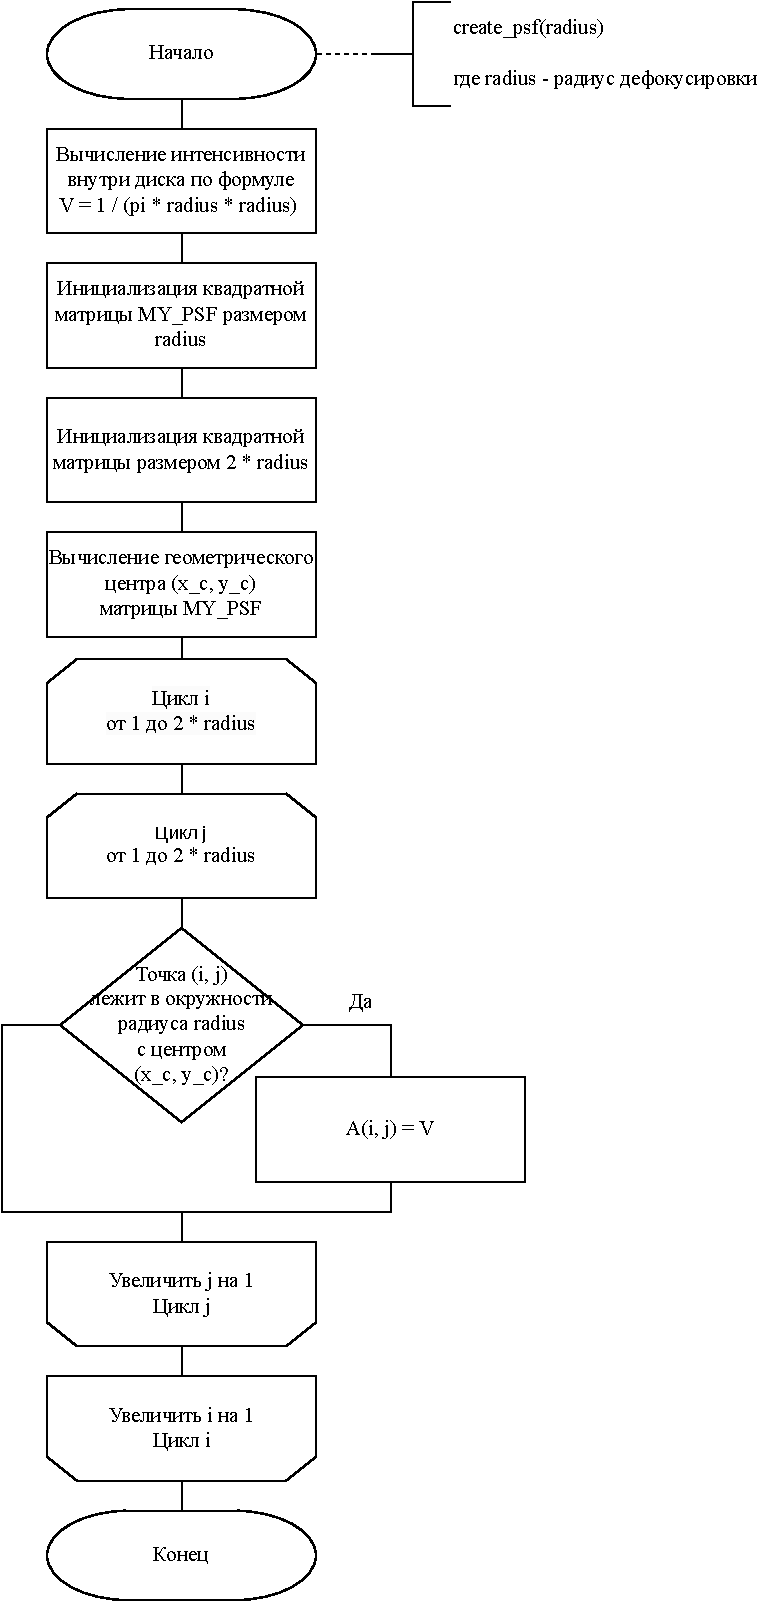
\includegraphics[scale=0.82]{assets/psf.pdf}
	\caption{Алгоритм вычисления ФРТ на основе радиуса дефокусировки}
	\label{psf}
\end{figure}

На \textit{четвертом} этапе производится деконволюция с использованием априорной информации методом Люси~---~Ричардсона. Т.к. этот алгоритм является классическим и не является объектом исследования, было принято решение не останавливаться подробно на реализации этого алгоритма.

На рисунке \ref{deconvolve} представлен алгоритм классической деконволюции на основе определенных параметров искажения.

\begin{figure}[H]
	\centering
	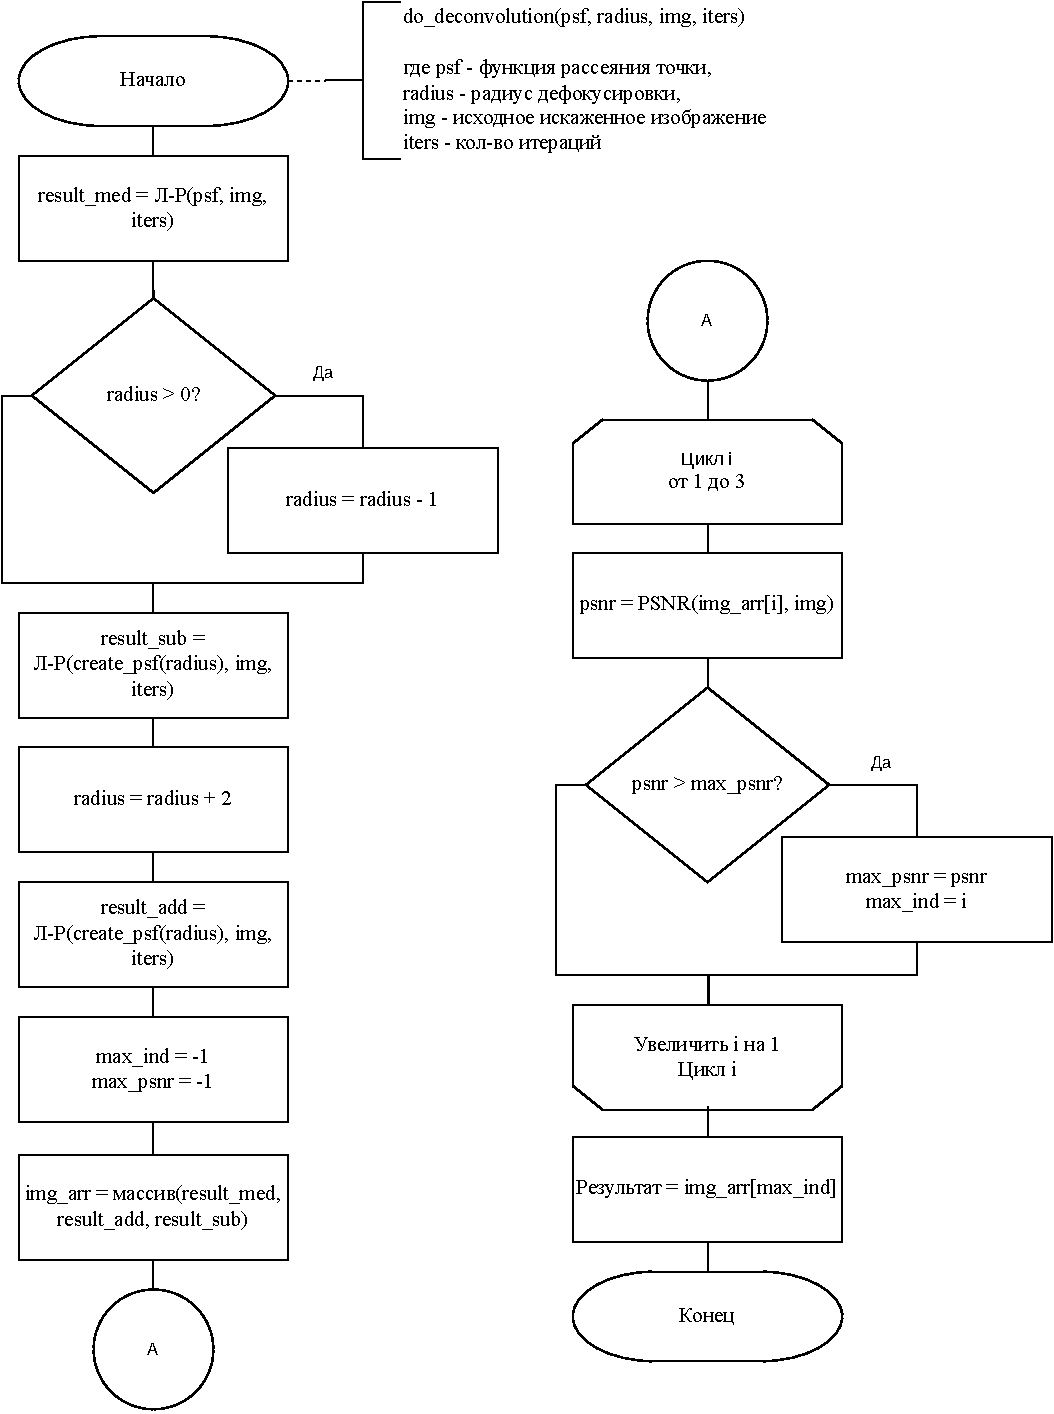
\includegraphics[scale=0.8]{assets/deconvolve.pdf}
	\caption{Алгоритм классической деконволюции на основе определенных параметров искажения}
	\label{deconvolve}
\end{figure}

Также было предложено варьировать на единицу в большую и меньшую сторону радиус дефокусировки, т.к. из-за наличия шума присутствует вероятность ошибиться на несколько пикселей с точностью вычисления радиуса. 

Для выбора наилучшего приближения из трех было предложено использовать метрику <<пиковое соотношение сигнал~--~шум>> (англ. PSNR --- Peak Signal Noise Ratio). Чем больше значение этой метрики, тем лучше произошло восстановление по предположению.

В рамках заключительного этапа входными параметрами являются радиус дефокусировки, ФРТ и исходное изображение, выходным --- матрица пикселей, соответствующая восстановленному изображению.

\subsection{Структура разрабатываемого программного обеспечения}

На рисунке \ref{struct} представлена диаграмма компонентов разрабатываемого программного обеспечения.

\begin{figure}[H]
	\centering
	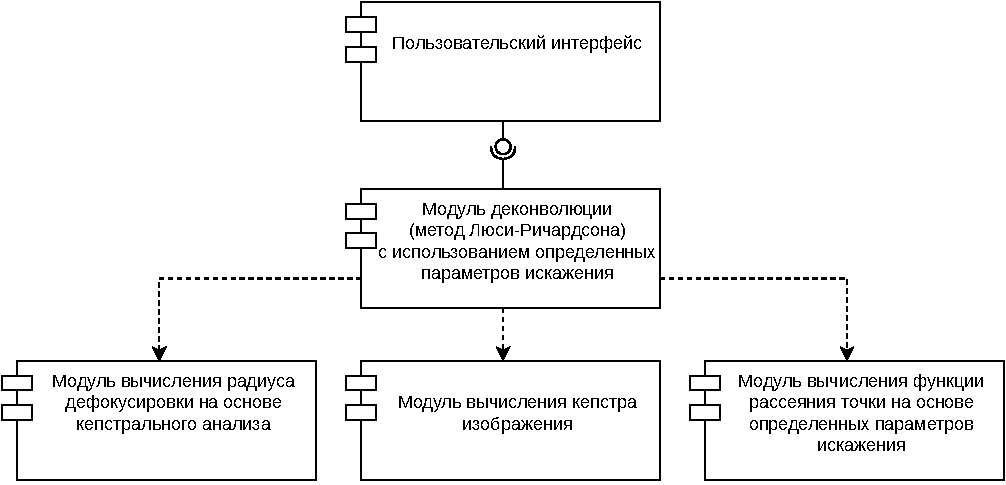
\includegraphics[scale=0.9]{assets/structure.pdf}
	\caption{Диаграмма компонентов разрабатываемого ПО}
	\label{struct}
\end{figure}

\section*{Выводы}

В данном разделе были сформулированы требования и ограничения к разрабатываемому методу и соответствующему ПО, рассмотрены основные этапы разрабатываемого метода в виде детализированной диаграммы IDEF0 и схем алгоритмов, а также спроектирована структура разрабатываемого ПО.